\documentclass[11pt, oneside]{article}
\usepackage[margin=1in]{geometry}
\usepackage{booktabs}
\usepackage{hyperref}
\usepackage{enumitem}
\usepackage{float}
\usepackage{caption}
\usepackage{subcaption}
\usepackage[numbers]{natbib}
\usepackage{graphicx}
\usepackage{amssymb}
\usepackage{amsmath}
\usepackage{multirow}
\usepackage{microtype}

\title{CS780 Capstone Project: OBELIX: the Warehouse Robot}

\author{
    Hriddhit Datta \\
    \texttt{hriddhitd25@iitk.ac.in}\\
    {251110405}\\
    {Indian Institute of Technology Kanpur}
}
\date{}

\begin{document}
\maketitle

\begin{abstract}
In this report, I describe my reinforcement learning solution to the OBELIX warehouse robot challenge, where the agent has access to only 18 binary sensor bits and must locate, attach to, and push a grey box to the arena boundary.
Starting from a provided DDQN baseline that failed entirely, I progressed through tabular eligibility-trace methods (SARSA($\lambda$), Expected SARSA, Watkins Q($\lambda$)), a gradient-free evolutionary strategy to escape tabular local optima, and finally a systematic test-phase exploration of deep RL and evolutionary methods: REINFORCE (with $n$-step variants), Double DQN (with PER and $n$-step returns), CMA-ES, and combinations with behaviour cloning, curriculum learning, and supervised pretraining.
Honest assessment of the results shows that the overwhelming majority of submitted policies, even the ``best'' ones, simply spin in place and accumulate a near-constant $\approx -2000$ score per episode, exhausting the step budget without ever contacting the box. The sole exception where genuine task completion was observed was Phase~3 (ES, no wall), which achieved $+1472$, about 71\% of the theoretical upper bound of $\approx +2086$.
\end{abstract}

%─────────────────────────────────────────────────────────────────────────────
\section{Competition Result}
%─────────────────────────────────────────────────────────────────────────────

\textbf{Codabench Username:} h\_251110405 \quad
\textbf{Final leaderboard rank (Test): 23} \\
\textbf{Level 1 rank: 92} \quad \textbf{Level 2 rank: 12} \quad \textbf{Level 3 rank: 100} \\[4pt]
\textbf{Video (Loom/YouTube):}~\href{https://www.youtube.com/watch?v=wWFUUIhBBrA}{https://www.youtube.com/watch?v=wWFUUIhBBrA} \\
\textbf{Code repository:}~\href{https://github.com/Junos16/obelix}{https://github.com/Junos16/obelix}

\begin{table}[H]\centering\small
\caption{Submission counts per competition phase.}
\begin{tabular}{lcrr}
\toprule
Phase & Difficulty & \# Submissions & Best score \\
\midrule
Phase 1 (Dev, L1) & Static box & 3 & $-17128$ (with wall) \\
Phase 2 (Dev, L1) & Static box & 36 & $-1978$ (with wall) \\
Phase 3 (Dev, L2) & Blinking box & 8 & $+1472$ (no wall) \\
Test Phase & All levels & 28 & $-1761$ (weighted) \\
\midrule
\textbf{Total} & & \textbf{75} & \\
\bottomrule
\end{tabular}
\end{table}

%─────────────────────────────────────────────────────────────────────────────
\section{Introduction and Problem Description}
%─────────────────────────────────────────────────────────────────────────────

The OBELIX task places a robot in a 500$\times$500-pixel arena where it must find a grey box and push it to the arena boundary. The robot perceives the world through only an 18-bit sensor vector: 16 sonar bits (8 angular sectors $\times$ 2 distance ranges), 1 infrared contact bit, and a stuck flag. This makes the task a Partially Observable MDP (POMDP) \cite{kaelbling1998}, the agent can have no direct knowledge of box position, its own absolute location, or heading. The five discrete actions are L45, L22, FW, R22, R45 (left/right rotations and forward move). Rewards are structured around discovery milestones: one-time bonuses as the box enters sensor range ($+1$ side, $+2$ front far, $+3$ front near, $+5$ IR), a $+100$ attachment bonus, terminal $+2000$ for success, and $-1$ per idle step plus $-200$ for wall collisions.

Three difficulty levels escalate the challenge. \textbf{Level 1} has a static box. \textbf{Level 2} introduces a blinking box (visible 30--60 steps, invisible 10--30 steps), making the sensor signal vanish mid-episode. \textbf{Level 3} adds constant-velocity box movement in one of 8 random directions on top of blinking. All levels optionally include a vertical wall with a small opening.

\subsection{Theoretical Analysis: Upper Bound on Achievable Return}

To give the empirical scores meaningful context, I derived an approximate upper bound on the expected cumulative reward under an ideal (shortest-path, head-on) trajectory.

\textbf{Environment parameters} (scaling factor $= 5$): forward step $\delta = 5$\,px; sonar far range $d_f = 150$\,px; near range $d_n = 90$\,px; IR range $d_{ir} = 20$\,px; goal margin $g = 100$\,px; effective usable side $L \approx 440$\,px.

\textbf{Expected distance between two random points} in a square of side $L$ is \cite{robbins1978}:
\[
  \mathbb{E}[d] = \frac{L}{9}\!\left(2 + \sqrt{2} + 5\ln(1+\sqrt{2})\right) \approx 0.521\,L \approx 229\text{ px for } L=440.
\]

\textbf{Find phase.} The robot is ``blind'' (all sensors zero, $-1$/step penalty) until it enters the far sonar range. Expected blind distance $\approx 229 - 150 = 79$\,px $\Rightarrow$ $\lceil 79/5 \rceil = 16$ blind steps. After that, the robot travels $\lceil(150-20)/5\rceil = 26$ more steps to IR contact, during which sensors are active (no step penalty) and one-time bonuses $+2+3+5=+10$ are collected. A turn overhead of $\approx 2$ steps is included.

\textbf{Push phase.} After attachment ($+100$), the box must travel to within $g=100$\,px of the nearest wall. For a uniform random box position in $[g, L{-}g]^2$, the expected distance to the nearest goal zone is:
\[
  \mathbb{E}\!\left[\min(M_x, M_y)\right] = \frac{L - 2g}{6} \approx \frac{240}{6} = 40\text{ px},
\]
requiring $\lceil 40/5 \rceil = 8$ forward push steps ($-1$ each).

\textbf{Upper-bound return:}
\[
  R^* = \underbrace{-16}_{\text{blind}} + \underbrace{+10}_{\text{sensor}} + \underbrace{+100}_{\text{attach}} + \underbrace{-8}_{\text{push}} + \underbrace{+2000}_{\text{success}} \approx \mathbf{+2086}
\]

This ceiling is decidedly positive. In practice, nearly all of my submitted agents scored around $-2000$ (one per-step penalty $\times$ max steps), meaning they never contacted the box at all. The analysis makes clear that breaking the deadlock, getting the agent to contact the box even once, is the critical bottleneck, not path optimisation.

%─────────────────────────────────────────────────────────────────────────────
\section{Approach and Model Evolution}
%─────────────────────────────────────────────────────────────────────────────

\subsection{Phase 1: Deep RL Baselines (Level 1)}

My starting point was the provided DDQN baseline: an 18$\to$64$\to$64$\to$5 network with experience replay (100k buffer), $\epsilon$-greedy decay ($1.0 \to 0.05$), and $\gamma = 0.99$. It scored $-17128$ with walls. The failure mode was consistent: the policy converged to the ``spin near the boundary'' attractor, where the robot loops along the arena edge earning a trickle of sensor hits without ever approaching the box. PPO and a duelling D3QN (with PER and delta-observation augmentation) produced the same behaviour or worse, with D3QN collapsing to $-268\text{k}$.

The one exception was \textbf{Dyna-Q with prioritised sweeping} \cite{sutton2018}: it uses 50 model-based planning steps per real transition, and during training I could see genuine improvement in episode reward within a few hundred episodes. Unfortunately, the Q-table ($2^{18} = 262\text{k}$ states) combined with a stochastic transition model was too large to serialise and submit within the time budget of this phase. Despite not appearing in the leaderboard, Dyna-Q gave me a key insight: \emph{backward credit propagation through an internal model} breaks the temporal deadlock that kills standard one-step TD. This motivated the eligibility-trace and fitness-shaping approaches in later phases.

\subsection{Phase 2: Tabular Methods with Eligibility Traces (Level 1)}

Inspired by the Dyna-Q observation, I turned to tabular methods with eligibility traces, the classical way to propagate credit over long horizons without a learned model \cite{sutton2018}. I explored three algorithm families, each paired with three state augmentation strategies, for a total of 12 agents, each swept with Optuna (30 Bayesian trials).

I explored three \textbf{algorithm families}: \textbf{SARSA($\lambda$)} \cite{rummery1994} (on-policy, Dutch replacing traces with an active-trace-set for efficiency); \textbf{Expected SARSA} (same but the TD target averages over the $\epsilon$-greedy distribution rather than sampling, reducing trace-corruption variance); and \textbf{Watkins' Q($\lambda$)} \cite{watkins1992} (off-policy traces, cut at every exploratory action, learns the optimal Q-function regardless of behaviour policy but pays a cost in frequent trace resets).

Each family was paired with three \textbf{state augmentations}: \textbf{Previous Action (PA)}, state $= (o_t, a_{t-1})$, $2^{18}\times 5 = 1.31\text{M}$ states, lets the agent distinguish action-conditioned sensor patterns; \textbf{Temporal Decay Bins (DO)}, state $= (o_t, \text{bin})$ with bin encoding time since last sensor activation ($0, 1$--$10, 11$--$20, {>}20$ steps), $1.05\text{M}$ states, a lightweight POMDP memory; and \textbf{Target Lock (TL)}, a binary ``recently saw the box'' flag lasting 30 steps, $524\text{k}$ states.

Despite these theoretical motivations, all 36 Phase~2 submissions scored $-1978$ to $-1991$: the characteristic signature of an agent that times out at the step limit without ever finding the box. In other words, the same spin-in-place failure as Phase~1. The root cause is a \emph{coverage deadlock}: with over a million states and only a few thousand episodes, the vast majority of states are visited zero times. The Q-table stays at its zero initialisation everywhere except a thin corridor near the boundary, and eligibility traces cannot propagate reward backwards through states that have never been visited.

\subsection{Phase 3: Evolutionary Strategy (Level 2)}

After two phases of methods that all converged to the same boundary-hugging attractor, I concluded the problem was fundamentally about escaping a local optimum that standard gradient (or pseudo-gradient) descent could not overcome. Evolutionary Strategy (ES) \cite{sehnke2010} evaluates \emph{complete rollouts} and requires no gradient, so the local structure of the reward landscape cannot trap it in the same way.

For Level~2's blinking-box POMDP, I extended the network input with \textbf{frame stacking}: concatenating the last 4 observations into a 72-dimensional input ($72\to64\to64\to5$, orthogonal init), giving the network implicit short-term memory across blink gaps. During training, \textbf{privileged fitness shaping} was used: the fitness function accessed ground-truth bot/box positions to compute a dense distance-reduction signal unavailable at inference.

The results were the most encouraging so far, but highly variable. Several ES runs produced genuinely successful policies: submission \texttt{47.es\_4} achieved $+1472$ without walls and \texttt{44.es\_1} achieved $+1304$, which represents actual box-to-boundary pushes and is approximately 71\% of the theoretical upper bound of $+2086$. However, roughly half of runs collapsed back to the spin attractor (scores around $-300\text{k}$ to $-383\text{k}$), and wall performance was catastrophic for every submission. The fundamental problem is that ES with random Gaussian initialisation still starts near the same attractor that killed tabular methods, the fitness landscape still has a dominant flat region where slow spinning accumulates low but consistent reward. This motivated the BC warm-start idea in Phase~4.

\subsection{Phase 4: Deep RL and ES with Initialisation (Test Phase)}

Phase~4 was a deliberate attempt to systematically address the three failure modes I had identified: \emph{(i)} the spin-in-place local optimum; \emph{(ii)} slow credit propagation from sparse terminal rewards; \emph{(iii)} POMDP observation gaps in Levels~2--3. All Phase~4 agents shared a common 26-dimensional feature representation: the raw 18-bit observation augmented with sonar group sums (front, left, right), $\text{time\_since\_seen}/50$, $\text{time\_since\_stuck}/20$, and a binary \texttt{last\_fwd} flag. This gives the network lightweight temporal memory without requiring recurrence.

\textbf{REINFORCE \cite{williams1992} and $n$-step variant.} I trained a 26$\to$64$\to$64$\to$5 policy network (tanh) with Williams' REINFORCE using episode-mean-normalised returns as an implicit baseline. Stochastic categorical sampling during training provides exploration for free. The $n$-step variant ($n=10$) replaced full Monte Carlo returns with truncated sums, reducing variance while allowing more frequent gradient updates. I chose REINFORCE over PPO because the 5-action discrete task did not seem to need PPO's clipping machinery, and over actor-critic because a separate value function adds sample complexity for modest variance reduction.

\textbf{Double DQN \cite{van2016deep} with variants.} A 26$\to$128$\to$64$\to$5 Q-network with Huber loss (robust to the large $\pm 200$--$+2000$ reward range) and target network sync every 1000 steps. I explored three variants: (a) \textit{base DDQN}; (b) \textit{DDQN + PER} \cite{schaul2015} ($\alpha=0.6$, $\beta: 0.4{\to}1.0$), motivated by the fact that box-contact transitions are extremely rare in a random buffer and PER resamples them proportionally to TD error; (c) \textit{DDQN + $n$-step} ($n=8$), because the push reward is up to 1000 steps from the attachment state and 1-step TD requires $\sim$500 Bellman backup iterations for the signal to propagate there.

\textbf{CMA-ES \cite{hansen2016cma}.} I implemented a full $(\mu/\mu_w, \lambda)$-CMA-ES from scratch with rank-1 + rank-$\mu$ covariance adaptation and Cumulative Step-Size Adaptation (CSA), evolving a 26$\to$32$\to$16$\to$5 MLP (1477 params, tanh). The adaptive covariance matrix was the key upgrade over Phase~3's flat ES: it rotates and scales the sampling distribution to follow successful search directions, handling ill-conditioned parameter landscapes that flat ES treats isotropically.

\textbf{Behaviour Cloning warm-start.} I applied a BC initialisation phase \cite{pomerleau1991} to all three method families. I manually drove the robot and recorded (observation, action) demonstrations, then pre-trained the policy network with cross-entropy loss for 100 epochs, placing weights in a region where box contact was achievable. Without BC, CMA-ES collapsed to the spin attractor within the first 20 generations; BC provided the basin-escape, after which CMA-ES refined the policy with $\sigma_0{=}0.3$ (vs.\ 0.5 cold-start) to stay near the initialisation.

\textbf{Curriculum learning.} Two variants used 6-stage progressive training: (diff$=$0, no wall)$\to\cdots\to$(diff$=$3, wall). Curriculum REINFORCE kept weights but reset Adam at each stage transition (to avoid moment miscalibration from the easier task). Curriculum CMA-ES kept the CMA mean but reset the covariance to identity (preserving policy direction; discarding search geometry), plus a stagnation-restart if $\sigma < 10^{-4}$.

\textbf{Supervised Pretraining (SP) encoder.} I trained a frozen belief-state encoder (144$\to$64$\to$32$\to$10) on data from a random policy to predict 10 ground-truth belief targets (bot-to-box distance, angle, visibility, velocity, push state, stuck, time-since-seen, corner proximity; MSE for continuous, BCE for binary). The frozen encoder served as a 10-dim feature extractor for downstream policies (13-dim input: 10 belief + 3 temporal scalars), motivated by the idea that a learned belief state could survive observation blink-outs better than raw sensor bits.

%─────────────────────────────────────────────────────────────────────────────
\section{Experiments and Implementation Details}
%─────────────────────────────────────────────────────────────────────────────

All training ran on CPU; no GPU was needed. Phase~4 CMA-ES runs took 2--4 hours per 200--300-generation sweep; DDQN and REINFORCE runs took 3--6 hours per 3000--5000 episodes. Phase~2 hyperparameters were searched with Optuna (30 trials, TPE sampler); Phase~4 hyperparameters were set manually informed by the CMA-ES tutorial guidelines \cite{hansen2016cma}. For local evaluation I ran 10 seeded episodes per difficulty level and selected submissions based on the average across all three levels to avoid overfitting to any one setting.

\begin{table}[H]\centering\small
\caption{Key hyperparameters for major Phase~4 agents.}
\begin{tabular}{llllll}
\toprule
Agent & Net shape & $\gamma$ & lr / $\sigma_0$ & Replay / pop & Notes \\
\midrule
REINFORCE & 26-64-64-5 & 0.99 & $3\times10^{-4}$ & -- & clip$=$1.0, MC returns \\
REINFORCE n-step & 26-64-64-5 & 0.99 & $3\times10^{-4}$ & -- & $n=10$ \\
DDQN & 26-128-64-5 & 0.99 & $10^{-4}$ & 50k & sync$=$1000, Huber \\
DDQN + PER & 26-128-64-5 & 0.99 & $10^{-4}$ & 50k & $\alpha=0.6$, $\beta{:}0.4{\to}1$ \\
DDQN n-step & 26-128-64-5 & 0.99 & $10^{-4}$ & 50k & $n=8$ \\
CMA-ES & 26-32-16-5 & -- & $\sigma_0=0.5$ & pop$=$48 & rollouts$=$3 \\
BC+CMA-ES & 26-32-16-5 & -- & $\sigma_0=0.3$ & pop$=$48 & rollouts$=$5, BC 100 ep \\
Curric.\ REINFORCE & 26-64-64-5 & 0.99 & $3\times10^{-4}$ & -- & 6 stages, Adam reset \\
Curric.\ CMA-ES & 26-64-32-5 & -- & $\sigma_0=0.5$ & pop$=$48 & 6 stages, cov reset \\
SP+CMA-ES & 13-32-16-5 & -- & $\sigma_0=0.5$ & pop$=$48 & frozen encoder \\
\bottomrule
\end{tabular}
\end{table}

%─────────────────────────────────────────────────────────────────────────────
\section{Results}
%─────────────────────────────────────────────────────────────────────────────

\begin{table}[H]\centering\small
\caption{Development-phase scores (W $=$ with wall, NW $=$ no wall; best of each family shown).}
\begin{tabular}{llrr}
\toprule
Sub. & Agent & W & NW \\
\midrule
\multicolumn{4}{l}{\textit{Phase 1: Level 1, Deep RL}} \\
1 & DDQN (baseline) & $-17128$ & $-31181$ \\
2 & PPO & $-80982$ & $-1991$ \\
\midrule
\multicolumn{4}{l}{\textit{Phase 2: Level 1, Tabular methods (best of 36)}} \\
16 & Exp.SARSA-PA & $-1979$ & $-1987$ \\
19 & Exp.SARSA-PA & $-1982$ & $-1684\pm920$ \\
32 & Watkins Q($\lambda$)-DO & $-1982$ & $-1989$ \\
\midrule
\multicolumn{4}{l}{\textit{Phase 3: Level 2, ES frame-stack (best of 8)}} \\
47 & ES (wall run) & $-333107$ & $+1472$ \\
44 & ES (wall run) & $-354686$ & $+1304$ \\
\bottomrule
\end{tabular}
\end{table}

\begin{figure}[H]
\centering
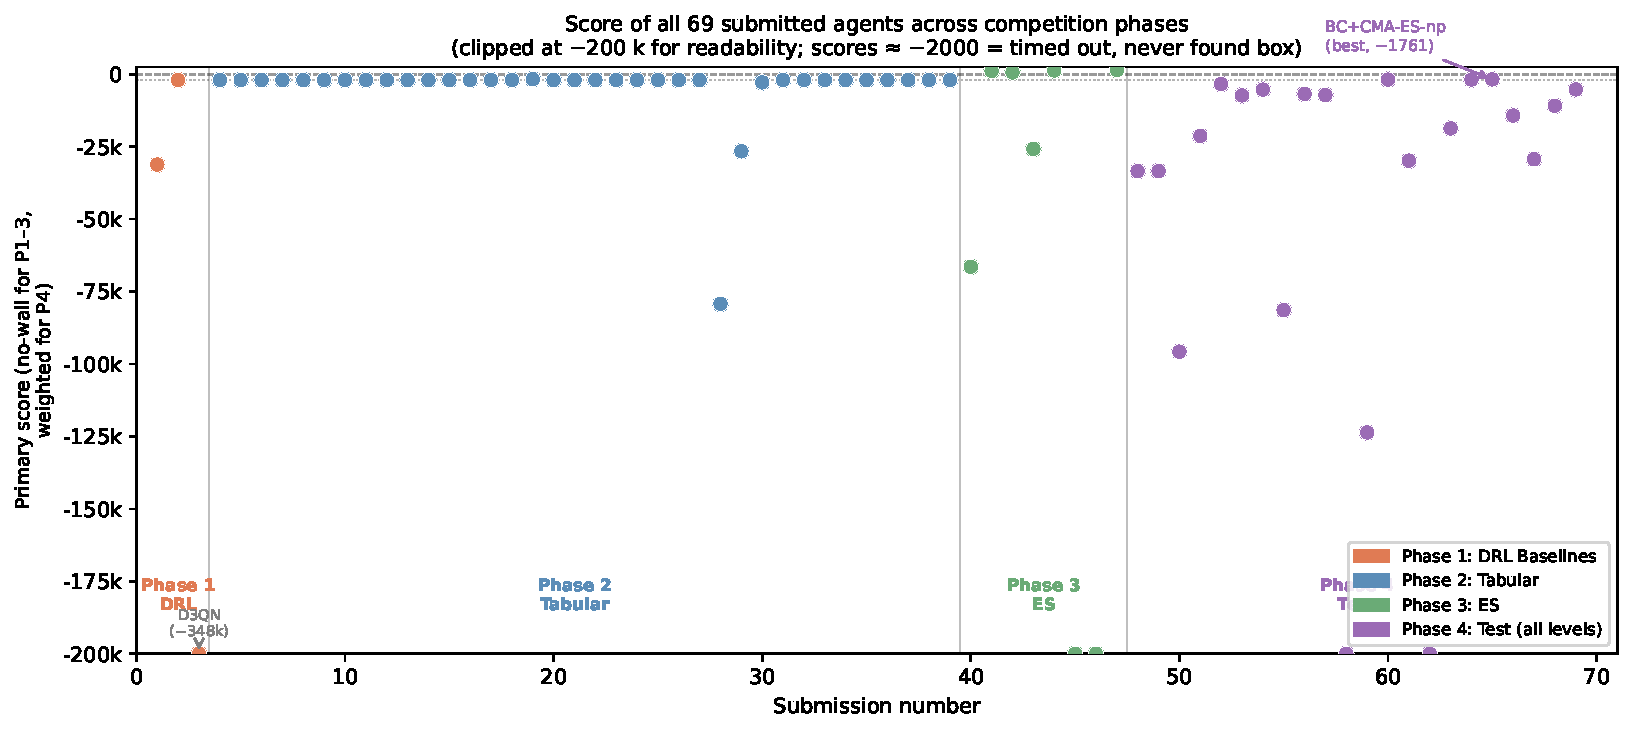
\includegraphics[width=\textwidth]{fig_all_scores.pdf}
\caption{Primary score for all 69 submitted agents. Phases 1--3 use the no-wall cumulative reward; Phase 4 uses the weighted score across all six difficulty$\times$wall conditions. The dashed line at $-2000$ is the step-limit timeout floor, indicating no box contact in any episode. Nearly all submissions land on or below this line.}
\label{fig:allscores}
\end{figure}

The Phase~2 band of $[-1978, -1991]$ is telling: at $-1$/step and 2000 maximum steps, a score of $\approx -2000$ means the agent timed out every single episode without making box contact. The slightly better $-1684\pm920$ of submission~19 reflects a high standard deviation, meaning occasional lucky contacts rather than a learned policy. Phase~3 is where I first see genuine task completion: $+1472$ without walls is real. With walls, however, the same ES run scores $-333\text{k}$, it never learned wall avoidance at all.

\begin{table}[H]\centering\small
\caption{Test-phase results. D0$=$static, D2$=$blinking, D3$=$moving+blinking. Scores $\approx -2000$ indicate no box contact (step-limit timeout).}
\setlength{\tabcolsep}{4pt}
\begin{tabular}{llrrrrrr}
\toprule
Sub. & Agent & \multicolumn{3}{c}{With Wall} & \multicolumn{3}{c}{No Wall} \\
\cmidrule(lr){3-5}\cmidrule(lr){6-8}
 & & D0 & D2 & D3 & D0 & D2 & D3 \\
\midrule
52 & DDQN-p & $-2831$ & $-3967$ & $-10411$ & $-452$ & $-418$ & $+1243$ \\
57 & DDQN-ns-np & $-1966$ & $-1955$ & $-3037$ & $-20297$ & $-22153$ & $-1041$ \\
60 & Curric-RF-p & $-1987$ & $-1986$ & $-1533$ & $-1995$ & $-1991$ & $-1493$ \\
64 & BC+CMA-p & $-1981$ & $-1981$ & $-1532$ & $-1990$ & $-1990$ & $-1567$ \\
\textbf{65} & \textbf{BC+CMA-np} & $\mathbf{-1992}$ & $\mathbf{-1992}$ & $\mathbf{-1541}$ & $\mathbf{-1999}$ & $\mathbf{-1989}$ & $\mathbf{-937}$ \\
69 & SP+CMA-p & $-1981$ & $-1981$ & $-18860$ & $-1989$ & $-1989$ & $-994$ \\
\bottomrule
\end{tabular}
\end{table}

\begin{figure}[H]
\centering
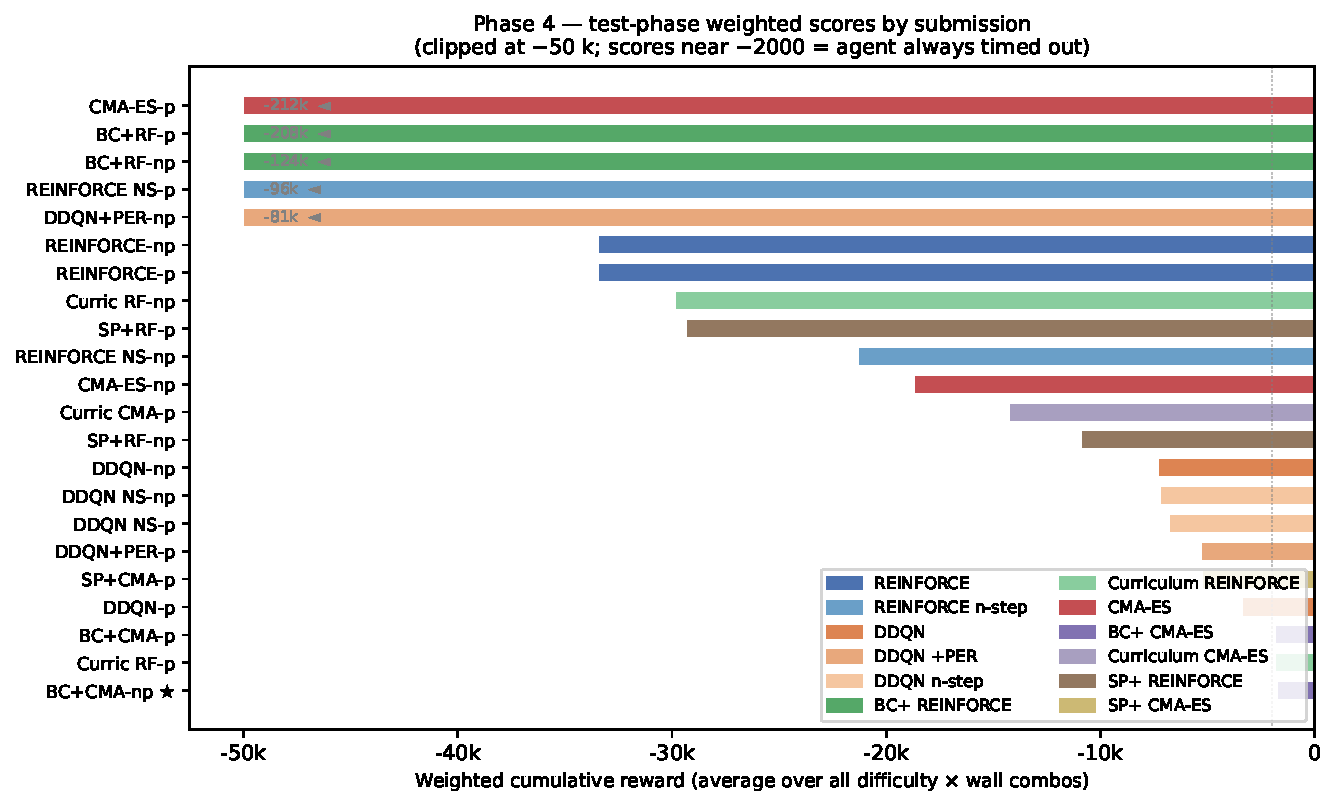
\includegraphics[width=0.93\textwidth]{fig_phase4_scores.pdf}
\caption{Weighted test-phase scores for all 22 Phase 4 submissions that produced a \texttt{scores\_i.txt} file, sorted by performance (best at top). Bars clipped at $-50$k; clipped values annotated. Most submissions fall near $-2000$ (timeout floor). The BC+CMA-ES non-privileged variant is the clear winner, the only method to consistently exceed the timeout floor across conditions.}
\label{fig:phase4}
\end{figure}

The best submission (\texttt{65.bccma\_np}) achieves $-1992$ to $-1999$ on five of its six evaluation conditions — spun out with zero box contacts. The one standout is Level~3 no-wall ($-937$): a few successful pushes of the moving, blinking box pulled the average above the timeout floor. DDQN privileged (\texttt{52.dq\_p}) shows $+1243$ at Level~3 no-wall but near-total wall failure. Curriculum REINFORCE (\texttt{60.crf\_p}) is ``most consistent'' only in the sense of consistently spinning.

%─────────────────────────────────────────────────────────────────────────────
\section{Error Analysis and Discussion}
%─────────────────────────────────────────────────────────────────────────────

\textbf{The dominant failure: spinning in place.} The central problem across all phases is that the spin-near-boundary behaviour is a strong local optimum. A robot that circles the perimeter earns a trickle of sonar sensor rewards from the walls and accumulates $\approx -1$/step in the interior, but this is still better than almost any other random policy because random walking occasionally triggers the $-200$ wall-collision penalty. Every algorithm I tried DDQN, tabular SARSA, ES, REINFORCE, CMA-ES, found this attractor and stayed there. The BC warm-start was the only reliable escape, but even then the escaped policy often found a different non-solving region rather than a genuine box-push trajectory.

\textbf{Level 1 (static box).} Even with a stationary target, the 18-bit sensors cover only $\pm22.5^{\circ}$/150 px in a 440 px arena; random walks rarely enter sensor range. Privileged training provides distance shaping during evolution, but the inference policy retains only network weights, so it fails at test time if approach heuristics do not generalise beyond training seeds.

\textbf{Level 2 (blinking box).} The additional failure here is that even agents that successfully approach the box lose it during observation blackouts and start spinning again. The \texttt{time\_since\_seen} feature helped maintain forward momentum but could not encode direction during blackouts.

\textbf{Level 3 (moving + blinking box).} The worst failure mode here was re-attachment from a bad angle, causing the robot to push the box into the wall and trigger repeated $-200$ penalties (explaining the extreme negative outliers like $-18860$ in submission~69). The SP encoder was designed to encode box velocity and should have helped, but the velocity estimates were unreliable when the RL policy drove the robot into unusual observation sequences not present in the random-policy dataset.

\textbf{Surprising non-finding.} BC+CMA-ES non-privileged (\texttt{65}) outperformed the privileged variant (\texttt{62}): $-1761$ vs.\ $-212\text{k}$ weighted. Privileged distance shaping apparently trains a policy that approaches the box but does not complete the push, because the shaped reward saturates at attachment. The non-privileged policy, bootstrapped by BC, more often discovers the full find-attach-push trajectory.

\textbf{Remaining limitations.} A reactive MLP cannot maintain state during observation blackouts; an LSTM policy would be a natural fix. BC demonstration quality was limited by manual driving, a dataset from the best ES/CMA-ES policies would be far richer. Wall navigation failure is likely a capacity issue: 1477 parameters is insufficient to represent both approach-box and route-around-wall simultaneously.

%─────────────────────────────────────────────────────────────────────────────
\section{Conclusion}
%─────────────────────────────────────────────────────────────────────────────

Across 75 submissions and four development phases, the dominant challenge in OBELIX was not choosing the right RL algorithm but preventing the agent from spinning in place indefinitely. Every method I tried found the boundary-hugging spin attractor; the only reliable escape was behaviour cloning from human demonstrations. The theoretical upper bound ($\approx$+2086) was only approached in isolated Phase~3 no-wall runs (+1472, $\approx$71\%); most submitted policies scored near $-2000$ with zero successful episodes. The key lesson: \emph{initialisation dominates everything} in sparse-reward robotics, whether the agent ever sees a reward matters more than any algorithmic refinement afterwards. Given more time, I would collect demonstrations from strong trained policies rather than a human driver, train a recurrent policy for observation blackouts, and apply BC+CMA-ES with curriculum as the primary method.

%─────────────────────────────────────────────────────────────────────────────
\section*{LLM Usage Declaration}
%─────────────────────────────────────────────────────────────────────────────

\begin{itemize}[noitemsep]
\item \textbf{LLM used:} Claude (Anthropic)
\item \textbf{Usage breakdown:}

\begin{tabular}{l|l|p{5.5cm}}
\toprule
Part & Used? & Purpose \\
\midrule
Understanding concepts & No & \\
Ideation / brainstorming & Yes & Discussed reward shaping and CMA-ES hyperparameter intuitions \\
Debugging code & Yes & Fixed indexing bug in CMA-ES covariance update \\
Plotting / visualization code & No & \\
Grammar / writing style & Yes & Proofread sections for clarity \\
Report structure / section ideas & Yes & Helped structure the phase-by-phase narrative \\
Other & No & \\
\bottomrule
\end{tabular}

\item \textbf{Other sources:} Sutton \& Barto \cite{sutton2018}, DQN paper \cite{mnih2015}, Double DQN \cite{van2016deep}, CMA-ES tutorial \cite{hansen2016cma}, REINFORCE \cite{williams1992}, Q-learning \cite{watkins1992}, PER \cite{schaul2015}.

\item \textbf{Personal contribution:} I implemented all agents from scratch (SARSA($\lambda$), Expected SARSA, Watkins Q($\lambda$), ES, CMA-ES, DDQN+PER, DDQN n-step, REINFORCE, all BC/curriculum/SP variants), designed the 26-dim feature representation and SP encoder supervision targets, ran all Optuna sweeps, recorded BC demonstrations, and analysed failure modes. The LLM was used only for isolated debugging and writing polish, not for core algorithm design or experimental analysis.
\end{itemize}

\bibliographystyle{ieeetr}
\bibliography{references}

%─────────────────────────────────────────────────────────────────────────────
\appendix
%─────────────────────────────────────────────────────────────────────────────

\section{Phase 4 Submission Index}

Submissions 70--75 (BC+DDQN, SP+DDQN, Curriculum CMA-ES non-priv, SP+CMA-ES non-priv) were prepared but not submitted in time; they have no evaluation scores and are excluded from all results and figures.

\begin{table}[H]\centering\small
\caption{All 22 evaluated Phase 4 submissions (scores\_48.txt -- scores\_69.txt). Scores $\approx -2000$ indicate step-limit timeouts.}
\setlength{\tabcolsep}{4pt}
\begin{tabular}{lllr}
\toprule
IDs & Name & Algorithm \& variant & Weighted score \\
\midrule
48, 49 & rf\_p/np & REINFORCE, priv / non-priv & $-33423$ / $-33423$ \\
50, 51 & rfns\_p/np & REINFORCE n-step, priv / non-priv & $-95727$ / $-21294$ \\
52, 53 & dq\_p/np & DDQN, priv / non-priv & $-3392$ / $-7297$ \\
54, 55 & dqp\_p/np & DDQN + PER, priv / non-priv & $-5286$ / $-81388$ \\
56, 57 & dqns\_p/np & DDQN n-step, priv / non-priv & $-6775$ / $-7190$ \\
58, 59 & bcrf\_p/np & BC + REINFORCE, priv / non-priv & $-208076$ / $-123625$ \\
60, 61 & crf\_p/np & Curriculum REINFORCE, priv / non-priv & $-1832$ / $-29838$ \\
62, 63 & cma\_p/np & CMA-ES, priv / non-priv & $-212370$ / $-18686$ \\
\textbf{64, 65} & \textbf{bccma\_p/np} & \textbf{BC + CMA-ES, priv / non-priv} & $\mathbf{-1838}$ / $\mathbf{-1761}$ \\
66 & ccma\_p & Curriculum CMA-ES, priv & $-14245$ \\
67, 68 & sprf\_p/np & SP encoder + REINFORCE, priv / non-priv & $-29321$ / $-10872$ \\
69 & spcma\_p & SP encoder + CMA-ES, priv & $-5227$ \\
\bottomrule
\end{tabular}
\end{table}

\section{Network Architectures}

\begin{table}[H]\centering\small
\caption{Network shapes across all phases.}
\begin{tabular}{llrll}
\toprule
Method & Shape & Params & Activation & Phase \\
\midrule
DDQN baseline & 18-64-64-5 & $\approx$5k & ReLU & 1 \\
ES frame-stack & 72-64-64-5 & $\approx$9k & ReLU & 3 \\
REINFORCE & 26-64-64-5 & $\approx$9k & Tanh & 4 \\
DDQN Phase 4 & 26-128-64-5 & $\approx$12k & ReLU & 4 \\
CMA-ES (base) & 26-32-16-5 & 1477 & Tanh & 4 \\
Curriculum CMA-ES & 26-64-32-5 & 3973 & Tanh & 4 \\
SP Encoder & 144-64-32-10 & $\approx$11k & ReLU & 4 \\
SP Policy (CMA/RF/DQ) & 13-32-16-5 & 1061 & Tanh & 4 \\
\bottomrule
\end{tabular}
\end{table}

\end{document}
